%versi 2 (8-10-2016)
\chapter{Dasar Teori}
\label{chap:Dasar Teori}
Pada bab ini akan diuraikan teori-teori yang berhubungan dengan pembangunan pohon kurikulum. Teori-teori tersebut adalah teori tentang pengertian graf,data terbuka, \textit{JSON}, \textit{DOT language}, dan visualisasi pohon menggunakan \textit{vis.js}.

\section{Graf}
\label{sec: Graf}

\subsection{Definisi Graf}
\label{sec: Definisi Graf}
Suatu graph didefinisikan oleh himpunan verteks dan himpunan sisi (edge).
Verteks menyatakan entitas-entitas data dan sisi menyatakan keterhubungan antara
verteks. Biasanya untuk suatu graf G digunakan notasi matematis. 
\begin{lstlisting}
G=(V,E)
G = Graph
V = Simpul atau vertex, atau node, atau titik
E = Sisi atau garis, atau Edge
\end{lstlisting}

V adalah himpunan \textit{verteks} dan E himpunan sisi yang terdefinisi antara pasangan-pasangan verteks. Sebuah sisi antara verteks x dan y ditulis {x, y}. Suatu graph H = (V1,E1) disebut subgraph dari graph G jika V1 adalah himpunan bagian dari V dan E1 himpunan bagian dari E.
\subsection{Istilah dalam Graf}
\label{sec: Istilah dalam Graf}
\begin{enumerate}
\item \textit{Incident}
Jika e merupakan busur dengan simpul-simpulnya adalah v dan w yang
ditulis e=(v,w), maka v dan w disebut "terletak" pada e, dan e disebut incident
dengan v dan w.
\item \textit{Degree}
Di dalam Graph ada yang disebut dengan \textit{Degree}, \textit{Degree} mempuyai 3 jenis antara lain :
\begin{itemize}
\item Degree dari suatu verteks x dalam undigraph adalah jumlah busur yang
incident dengan simpul tersebut.
\item Indegree dari suatu verteks x dalam digraph adalah jumlah busur yang
kepalanya incident dengan simpul tersebut, atau jumlah busur yang "masuk" atau menuju simpul tersebut.
\item Outdegree dari suatu verteks x dalam digraph adalah jumlah busur yang
ekornya incident dengan simpul tersebut, atau jumlah busur yang "keluar"
atau berasal dari simpul tersebut.
\end{itemize}
\item \textit{Adjacent}
Pada graph tidah berarah, 2 buah simpul disebut adjacent bila ada busur yang
menghubungkan kedua simpul tersebut. Simpul v dan w disebut adjacent. 
Pada graph berarah, simpul v disebut adjacent dengan simpul w bila ada busur
dari w ke v.
\item \textit{Successor dan Predecessor}
Pada graph berarah, bila simpul v \textit{adjacent} dengan simpul w, maka simpul v adalah \textit{successor} simpul w, dan simpul w adalah \textit{predecessor} dari simpul v.
\end{enumerate}

\section{Data Terbuka}
\label{sec: Data Terbuka}
Teknologi sekarang memungkinkan untuk membangun layanan yang menjawab pertanyaan-pertanyaan secara otomatis. Sebagian besar data yang diperlukan untuk menjawab pertanyaan-pertanyaan dihasilkan oleh badan-badan publik. Namun, seringkali data yang diperlukan belum tersedia dalam bentuk yang mudah digunakan. Gagasan dari data terbuka mengarah kepada informasi di mana setiap orang bebas untuk mengakses dan menggunakan ulang untuk berbagai tujuan - sudah bergulir dalam beberapa tahun ini.  	

\subsection{Apa itu Data Terbuka}
\label{sec: Apa itu Data Terbuka}
Data terbuka adalah data yang dapat digunakan secara bebas, dimanfaatkan, dan didistribusikan kembali oleh siapapun tanpa syarat, kecuali dengan mengutip sumber dan pemilik data. Selain itu, seluruh data yang dipublikasikan harus mengikuti peraturan perundang-undangan yang berlaku. Kriteria penting dari data terbuka adalah:
\begin{enumerate}
\item Ketersediaan dan Akses
Data harus tersedia utuh dan bebas biaya. Akan lebih baik jika data dapat diunduh melalui internet. Data juga harus tersedia dalam bentuk yang mudah digunakan dan dapat diolah kembali.
\item Penggunaan dan Pendistribusian 
Data yang digunakan dan didistribusikan kembali harus memenuhi syarat-syarat yang telah ditentukan.
\item Partisipasi Universal
Setiap orang bebas menggunakan dan mendistribusikan kembali \textit{dataset}. Tidak diperkenankan adanya diskriminasi atas bidang usaha, orang, atau kelompok.
\end{enumerate}

Semua kriteria yang ada di dalam data terbuka sangat penting karena menunjukkan kejelasan tentang apa yang dimaksud dengan terbuka itu sendiri. Istilah yang digunakan untuk menjelaskan ketiga kriteria data terbuka adalah \textit{interoperabilitas}. Interoperabilitas sangat penting karena memungkinkan komponen-komponen yang berbeda untuk bisa bekerja sama. Kemampuan untuk mengkomponenisasi komponen-komponen sangatlah esensial untuk membangun sistem yang besar dan kompleks. Tanpa \textit{interoperabilitas} hal ini menjadi tidak mungkin di mana kemampuan untuk berkomunikasi (lintas operasi) sangat berpengaruh terhadap keberhasilan suatu rencana.

Inti dari sebuah "keumuman" \textit{data} merupakan salah satu bagian dari materi "terbuka". \textit{Interoperabilitas} ini merupakan komponen penting untuk merealisasikan praktik utama manfaat dari "keterbukaan": Peningkatan dramatis kemampuan untuk mengkombinasikan sekumpulan data berbeda secara bersama-sama sehingga merangsang pengembangan produk dan layanan yang lebih baik. keterbukaan dapat memastikan bahwa ketika ada dua kumpulan data dari dua sumber berbeda, maka kita dapat menggabungkan data tersebut secara bersama-sama, dan memastikan bahwa data yang kita dapat informasinya benar.

\subsection{Mengapa Data Terbuka}
\label{sec: Mengapa Data Terbuka}
Data terbuka adalah sumber daya luar biasa yang belum dimanfaatkan sepenuhnya. Banyak individu dan organisasi mengumpulkan berbagai jenis data berbeda dalam rangka untuk melakukan tugas mereka. Pemerintah sangat signifikan dalam hal ini, tidak hanya karena kuantitas dan sentralitas dari data yang dikumpulkan, tetapi juga karena sebagian besar dari data pemerintah adalah bersifat publik secara hukum, dan oleh karena itu bisa dibuat terbuka dan tersedia untuk orang lain untuk dipergunakan. hal itu menjadi menarik karena banyak individu atau kelompok yang ingin mengetahui data yang ada. 

Ada banyak area di mana kita bisa mengharapkan data terbuka untuk menjadi sebuah nilai, dan menjadi contoh bagaimana data terbuka telah digunakan. Ada juga kelompok dengan banyak orang berbeda dan organisasi yang dapat meraih keuntungan dari ketersediaan data yang terbuka, termasuk pemerintah itu sendiri. Pada saat yang sama adalah mustahil untuk memprediksi secara tepat bagaimana dan di mana nilai akan dibuat di masa depan. Sifat alami dari inovasi adalah bahwa pengembangan seringkali datang dari tempat yang tidak mungkin. Hal ini sudah dimungkinkan dengan merujuk pada sejumlah data terbuka yang telah menciptakan nilai. Beberapa nilai ini meliputi: 
\begin{itemize}
\item Transparansi dan kendali
\item Partisipasi
\item Penguatan mandiri
\item Inovasi
\item Efisiensi dan Efektivitas lebih baik dari layanan yang sudah ada
\item Pengukuran pengaruh dari kebijakan-kebijakan
\item Pengetahuan baru dari kombinasi sumber data dan pola-pola dalam volume data yang besar
\end{itemize}

\subsection{Cara Membuka Data}
\label{sec: Cara Membuka Data}
Data Terbuka dapat dibuka para pemegang data. Para pemegang data dapat melakukannya secara mendasar, tetapi juga mencakup masalah-masalah yang tersembunyi dan menjebak. Terdapat tiga aturan kunci yang kami rekomendasikan saat membuka data:
\begin{enumerate}
\item Jadikan lebih praktis.
\item Terlibat dari awal dan melibatkan diri sesering mungkin.
\item Mengatasi kekhawatiran umum dan kesalahpahaman. 
\end{enumerate}

Ada empat langkah utama dalam membuat data terbuka, yang masing-masing akan dibahas secara rinci di bawah ini. Langkah-langkah tersebut adalah yang paling memungkinkan - banyak dari langkah-langkah tersebut dapat dilakukan secara bersamaan. 
\begin{enumerate}
\item \textbf{Pilih Kumpulan Data(s}) \\
Pemilihan kumpulan-kumpulan data(s) yang direncanakan untuk menjadikannya terbuka merupakan langkah pertama – meskipun perlu diingat bahwa seluruh proses pembukaan data akan berulang dan dapat kembali ke langkah ini bila mengalami masalah di kemudian hari. Jika sudah mengetahui persis kumpulan-kumpulan data(s) maka dapat merencanakan untuk dibuka dan dapat langsung ke bagian berikutnya. Bagaimanapun juga, dalam banyak kasus, terutama untuk lembaga-lembaga yang besar, untuk berfokus pada memilih kumpulan data menjadi sebuah tantangan. 
\item \textbf{Menerapkan sebuah Lisensi Terbuka (Keterbukaan Resmi)} \\
Di kebanyakan yurisdiksi terdapat hak kekayaan intelektual di dalam data yang mencegah pihak ketiga dari penggunaannya, penggunaan ulang dan pendistribusian data tanpa izin eksplisit. Bahkan di tempat di mana keberadaan hak hukum serba tidak pasti, penting untuk menerapkan lisensi demi sebuah kejelasan. Dengan demikian, jika kita berencana untuk membuat data tersedia, maka harus menaruh lisensi di atasnya dan jika data menjadi terbuka ini bahkan lebih penting lagi. 
\item \textbf{Menjadikan Data Terseddia}\\
Data terbuka membutuhkan keterbukaan secara teknis sebagaimana keterbukaan yang resmi secara hukum. Khususnya, data harus bisa tersedia secara masal dalam format (yang dapat dibaca mesin).
\begin{itemize}
\item \textbf{Available} \\
Data seharusnya dihargai tidak lebih dari biaya reproduksi yang wajar, sebaiknya dijadikan sebagai unduhan gratis dari internet. Model penghargaan ini dapat dicapai karena lembaga anda tidak perlu menangani biaya apapun saat menyediakan data untuk digunakan.
\item \textbf{In Bulk}\\
Data harus tersedia dalam kumpulan yang lengkap. Jika anda memiliki daftar yang dikoleksi di bawah aturan undang-undang, seluruh daftar tersebut harus tersedia untuk diunduh.
\item \textbf{In an open, machine-readable format}\\
Penggunaan-ulang data yang disediakan oleh sektor publik tidak seharusnya tunduk pada pembatasan paten. 
\item \textbf{Jadikan hingga Mudah untuk ditemukan} \\
terbitkan di web dan mungkin kelola sebuah pusat katalog untuk membuat daftar dari kumpulan data terbuka.
\end{itemize}
\end{enumerate}

\section{\textit{JSON}}
\label{sec: JSON}

JSON \textit{(JavaScript Object Notation)} adalah format pertukaran data. JSON merupakan format teks yang tidak bergantung pada bahasa pemprograman apapun. Kenapa \textit{JSON}? Karena ukuran datanya lebih kecil dibanding dengan XML, sifatnya \textit{"self-describing"} dan mudah dimengerti. Formatnya berbasis teks dan terbaca manusia serta digunakan untuk mempresentasikan struktur data sederhana. Format teks dari JSON itu sendiri identik dengan kode untuk membuat objek \textit{JavaScript} memiliki kesamaan dengan Java Script, hanya saja JSON lebih mudah dimengerti. 

\subsection{Struktur JSON}
\label{sec: Struktur JSON}
JSON terbuat dari dua struktur:
\begin{enumerate}
\item Kumpulan pasangan nama/nilai. Pada beberapa bahasa, hal ini dinyatakan sebagai objek \textit{(object)}, rekaman \textit{(record)}, struktur \textit{(struct)}, kamus \textit{(dictionary)}, tabel hash\textit{(hash table)}, daftar berkunci \textit{(keyed list)}, atau \textit{associative array}.
\item Daftar nilai terurutkan \textit{(an ordered list of values)}. Pada kebanyakan bahasa, hal ini dinyatakan sebagai larik \textit{(array)}, vektor \textit{(vector)}, daftar \textit{(list)}, atau urutan \textit{(sequence)}. 
\end{enumerate}

\textit{JSON} menggunakan bentuk sebagai berikut:
\begin{enumerate}
\item \textbf{Objek} adalah sepasang nama/nilai yang tidak terurutkan. Objek dimulai dengan { (kurung kurawal buka) dan diakhiri dengan } (kurung kurawal tutup). Setiap nama diikuti dengan : (titik dua) dan setiap pasangan nama/nilai dipisahkan oleh , (koma).
\begin{figure}[H]
		\centering
		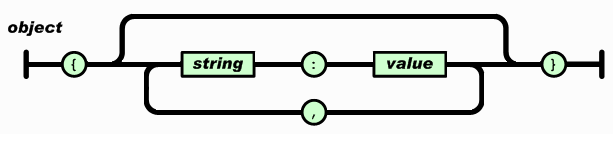
\includegraphics[scale = 0.5]{1.png}
		\caption{Objek}
		\label{}
\end{figure}	

\item \textbf{Larik} adalah kumpulan nilai yang terurutkan. Larik dimulai dengan [ (kurung kotak buka) dan diakhiri dengan ] (kurung kotak tutup). Setiap nilai dipisahkan oleh , (koma).
\begin{figure}[H]
		\centering
		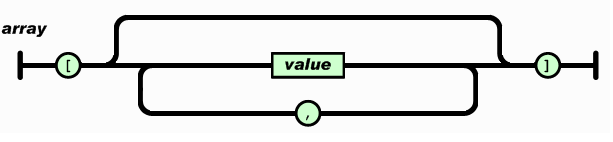
\includegraphics[scale = 0.5]{2.png}
		\caption{Larik}
		\label{}
\end{figure}	

\item \textbf{Nilai}, dapat berupa sebuah \textit{string} dalam tanda kutip ganda, atau angka, atau true atau false atau null, atau sebuah objek atau sebuah larik. Struktur-struktur tersebut dapat disusun bertingkat.
\begin{figure}[H]
		\centering
		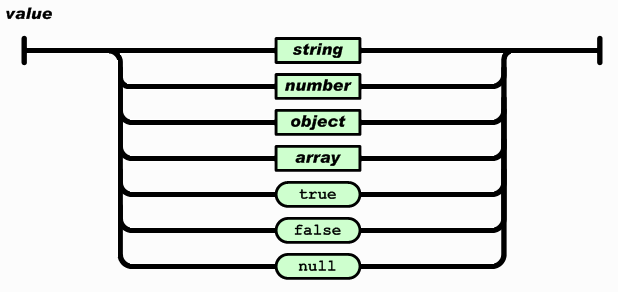
\includegraphics[scale = 0.5]{3.png}
		\caption{Nilai}
		\label{}
\end{figure}	


\end{enumerate}

\subsection{Contoh Sintaks}
\label{sec: Contoh Sintaks}
Contoh berikut menunjukkan representasi JSON untuk suatu objek yang mendeskripsikan seseorang.
\begin{lstlisting}
{ 
"namaDepan": "Budi", 
"namaBelakang": "Subudi", 
"alamat": { 
	"namaJalan": "Jl. Sudirman 15A", 
	"kota": "Jakarta Selatan", 
	"provinsi": "DKI Jakarta", 
	"kodePos": 11111 }, 
	"nomerTelepon": [ 
	"021 555-1234", 
	"021 555-4567" 
	] 
}
\end{lstlisting}




\section{DOT Language}
\label{sec: DOT Language}
\textit{DOT} adalah bahasa yang dapat digunakan untuk menampilkan grafik secara teks, sehingga dapat diproses melalui titik untuk membuat grafik sebagai representasi grafis dalam format yang berbeda seperti .ps, .pdf, dll. DOT telah dikembangkan sebagai bagian dari proyek \textit{Graphviz}, yang merupakan kumpulan alat untuk visualisasi grafik. 

\subsection{Dasar Menggambar Graf}
\label{sec: Dasar Menggambar Graf}
Dot mengambil empat langkah utama dalam menggambar grafik. Langkah pertama menetapkan diskrit peringkat ke node dalam gambar atas ke bawah, menentukan peringkat di koordinat Y. Tepi yang membentang lebih banyak dari satu peringkat dipecah menjadi rantai simpul dan tepi unit. Langkah kedua \textit{node} dalam barisan untuk menghindari penyeberangan. Langkah ketiga menetapkan koordinat \textit{node} X untuk disimpan dibaris terpendek. Langkah terakhir rute tepi splines. Grafik menggunakan dot memiliki tiga jenis \textit{item}: grafik, simpul, dan tepi. Grafik sendiri memiliki dua bentuk yaitu grafik (tidak diarahkan) atau digraph (diarahkan). Karena dot membuat \textit{layout} grafik yang diarahkan maka contoh dalam kasus ini menggunakan digraph. 

Gambar graph1 adalah contoh grafik dalam bahasa dot. Baris 1 memberi nama dan jenis grafik. Baris berikut membuat node, tepi, atau subgraf, dan atur atribut. Nama merupakan identifier C, nomor, atau kutipan C. Sebuah simpul diciptakan pertama kali namanya muncul di \textit{file}. Tepian dibuat saat node berada bergabung dengan operator tepi ->. Pada contoh, baris 2 membuat tepi lalu mengurai dari \textit{parse} ke \textit{execute}. Untuk menjalankan dot pada file ini (dimisalkan graph1.dot) dapat mengetikan $ dot -Tps graph1.dot -o graph1.ps $ dan akan menghasilkan gambar graph1. 
\begin{lstlisting}
1: digraph G {
2: main -> parse -> execute;
3: main -> init;
4: main -> cleanup;
5: execute -> make_string;
6: execute -> printf
7: init -> make_string;
8: main -> printf;
9: execute -> compare;
10: }
\end{lstlisting}

\begin{figure}[H]
		\centering
		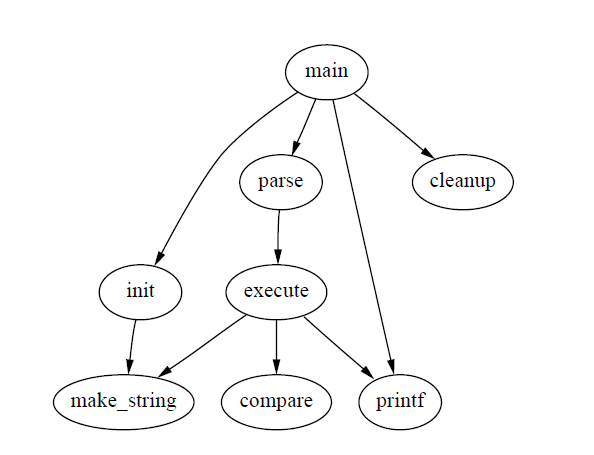
\includegraphics[scale = 0.5]{graph1.png}
		\caption{Gambar Graph1}
		\label{}
\end{figure}	

\subsection{Atribut Menggambar}
\label{sec: Atribut Menggambar}
Dalam membuat graf dibutuhkan beberapa atribut untuk menyempurnakan gambar. Atribut tersebut berisi 
\begin{enumerate}
\item Bentuk dan Label.\\
Pada bentuk dan label nantinya akan ditentukan \textit{node} akan berbentuk apa dan label pada node akan berisi apa. Secara \textit{default} bentuk dari node sendiri adalah elips. Tetapi ada bentuk lain yang diberikan untuk \textit{node} yaitu kotak, lingkaran, polygon, dll. 
\item Tampilan Graf\\
Simpul dan tepi memiliki atribut warna dan gaya. Penggunaan warna dalam membuat graf memiliki beberapa syarat. Pertama hindari menggunakan terlalu banyak warna cerah. Kedua, ketika node dipenuhi warna gelap label nampaknya lebih mudah dibaca dengan \textit{fontcolor} = putih dan \textit{fontname} = \textit{Helvetica}. Ketiga, menentukan ruang warna dengan mendefinisikan \textit{nodecolor}, \textit{edgecolor}, atau \textit{graphcolor} dalam file library. Misalnya, untuk menggunakan warna RGB, letakkan baris berikut di file lib.ps. / nodecolor {setrgbcolor} bind def. Gunakan opsi baris perintah -l untuk memuat file ini. $ dot -Tps -l lib.ps file.dot -o file.ps $
\item Ukuran Gambar dan Jarak\\
Seringkali gambar yang dibuat dengan ukuran dan pemisahan \textit{nodes default} terlalu besar untuk target atau untuk ruang yang diizinkan untuk gambar dalam dokumen. Ada beberapa cara untuk mencoba mengatasi masalah ini. Pertama, melihat bagaimana titik pada ukuran tata letak akhir. Tata letak awalnya dibuat secara internal dengan ukuran awal, dengan menggunakan pengaturan \textit{default}. Secara default, \textit{nodes} paling sedikit 0,75 inci dengan lebar 0,5; \textit{font} adalah 14, \textit{nodes} dipisahkan paling sedikit 0,25 dan diberi peringkat oleh 0,5 Tidak ada batasan ukuran atau aspek rasio gambar, jadi jika grafiknya besar, tata letaknya juga besar. Jika tidak menentukan ukuran atau rasio, maka ukuran awal akan dicetak. Cara termudah untuk mengontrol ukuran output gambar adalah dengan mengatur ukuran = x; y pada file grafik (atau pada baris perintah menggunakan -G). Ini menentukan kotak pembatas tata letak akhir. 
\end{enumerate}

Tabel untuk atribut menggambar sebagai berikut
\begin{figure}[H]
		\centering
		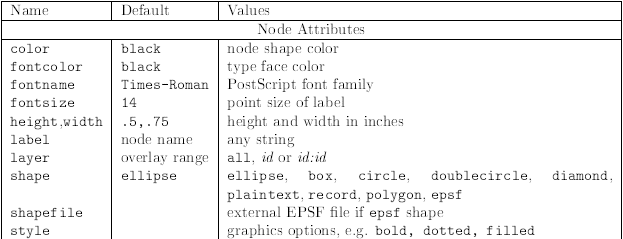
\includegraphics[scale = 0.5]{NodeA.png}
		\caption{node attributes}
		\label{}
\end{figure}	

\begin{figure}[H]
		\centering
		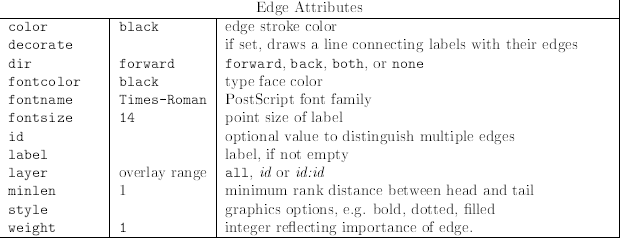
\includegraphics[scale = 0.5]{EdgeA.png}
		\caption{edge attributes}
		\label{}
\end{figure}	

\begin{figure}[H]
		\centering
		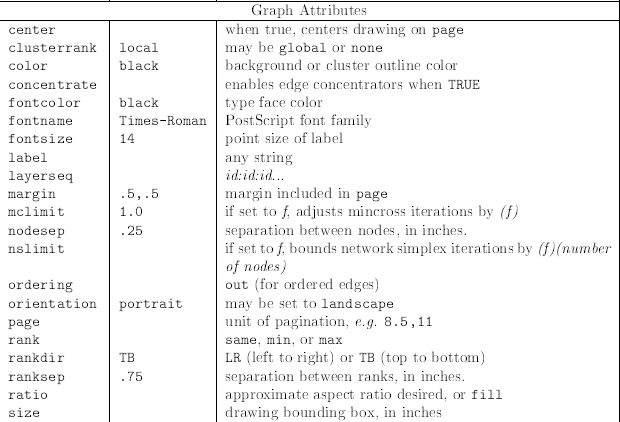
\includegraphics[scale = 0.5]{GrafA.png}
		\caption{graph attributes}
		\label{}
\end{figure}	


\subsection{Subgraf dan Pengelompokan}
\label{sec: Subgraf dan Pengelompokan}
Subgraf memiliki tiga peran di \textit{Graphviz}. Pertama, subgraf dapat digunakan untuk mewakili struktur grafik, yang menunjukkan bahwa simpul dan tepi tertentu harus dikelompokkan bersama. Informasi pada subgraf ditentukan secara semantik tentang komponen grafik. Tepi dibuat dari setiap simpul di sebelah kiri ke setiap simpul di sebelah kanan. Contohnya sebagai berikut 
\begin{lstlisting}
A -> {B C} 

sama dengan
A -> B
A -> C
\end{lstlisting}

Kedua, subgraf dapat memberikan konteks untuk mengatur atribut. Sebagai contoh, sebuah subgraf dapat menentukan bahwa warna biru adalah warna \textit{default} untuk semua node yang didefinisikan di dalamnya. Dalam konteks gambar grafik, contohnya sebagai berikut

\begin{lstlisting}
subgraf {
peringkat = sama; A; B; C;
}
\end{lstlisting}

Subgraf ini menentukan bahwa simpul A, B dan C semuanya harus ditempatkan pada rangking yang sama jika ditarik menggunakan titik.

Ketiga untuk subgraf secara langsung melibatkan bagaimana grafik akan ditata oleh mesin. Jika nama subgraf dimulai dengan \textit{cluster}, \textit{Graphviz} mencatat subgraf sebagai subgraf \textit{cluster} khusus. Jika didukung, mesin akan melakukan tata letak sehingga simpul milik cluster digambar bersama, dengan keseluruhan gambar cluster yang ada di dalam persegi panjang yang melintang. Subgraf \textit{cluster} bukan bagian dari bahasa DOT, namun hanya konvensi sintaks yang dipatuhi oleh mesin.  

\section{Visualisasi Graf dengan Viz.js}
\label{sec: Visualisasi Graf dengan Viz.js}
Data terbuka adalah data yang terbuka. Tetapi jika dilihat lagi data terbuka yang dimaksud dalam konteks saat ini adalah data yang bebas diakses, data yang bebas digunakan kembali, dan data dalam format \textit{machine-readable}. Data yang bebas diakses dan bebas digunakan kembali sudah cukup jelas. Semua orang boleh dan diizinkan untuk mengakses dan menggunakan data tersebut untuk keperluannya masing-masing. Pada dasarnya data dalam format PDF, image, atau apapun yang bisa dilihat oleh manusia jika masuk ke dalam kriteria ini. Namun bisa dilihat dan dimengerti saja tidak cukup. Maka dari itu ada kriteria ketiga yaitu "data dalam format \textit{machine-readable}". Format \textit{machine-readable adalah} sebuah format yang memiliki struktur jelas, di mana satu data berada pada satu baris, dan dalam format terbuka (contohnya format CSV atau JSON). Tujuannya satu, agar data yang ada bisa dimengerti oleh mesin. Dalam hal ini komputer. Jika data dapat dimengerti oleh komputer, maka pengolahan data akan lebih baik, lebih cepat, lebih efisien dan lebih akurat.

JSON sebagai salah satu format terbuka digunakan untuk membuat graf. Graf ini dihasilkan dengan menggunakan \textit{viz.js} yang merupakan mesin pembaca \textit{DOT}. \textit{DOT} sendiri dibuat mdengan melihat struktur JSON. Penulisan \textit{viz} sebagai visualisi graf itu sendiri sebgai berikut
\begin{lstlisting}
Viz(src, options={ format="svg", engine="dot", scale, images=[{ path, width, height }], totalMemory=16777216 })
\end{lstlisting}
\begin{itemize}
\item \textit{src} adalah string yang mewakili grafik yang akan ditampilkan dalam bahasa \textbf{DOT}.
\item \textit{options} \\
\begin{itemize}
\item \textit{format} menetapkan \textit{format} keluaran, dan hasilnya salah satu dari "svg", "xdot", "plain", "ps", "json", atau "png-image-element". 
\item \textit{engine}, mengatur mesin \textit{Graphviz} untuk digunakan, salah satunya "circo", "dot", "fdp", "neato", "osage", or "twopi".
\item \textit{scale}, menetapkan faktor skala untuk format "png-image-element".
\item \textit{images}, menentukan dimensi gambar untuk digunakan saat membuat nodes dengan atribut gambar. 
\item \textit{file}, menentukan file yang tersedia untuk \textit{Graphviz} menggunakan \textit{file system} dalam memori. Ini adalah array dari objek, {path, data}. File dibuat terhadap direktori kerja.
\item \textit{total memory}, mengatur memori yang tersedia.
\end{itemize}

\end{itemize}